\subsection{State of the art: the search for \bbonu\ decays}
\label{sec.state}

\begin{figure}[thb!]
\centering
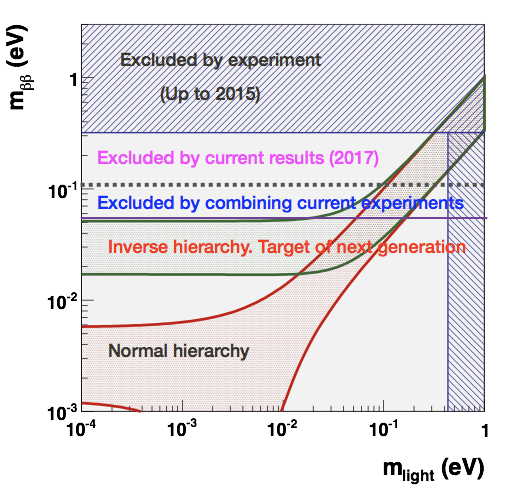
\includegraphics[width=0.55\textwidth]{img/landscape.png}
%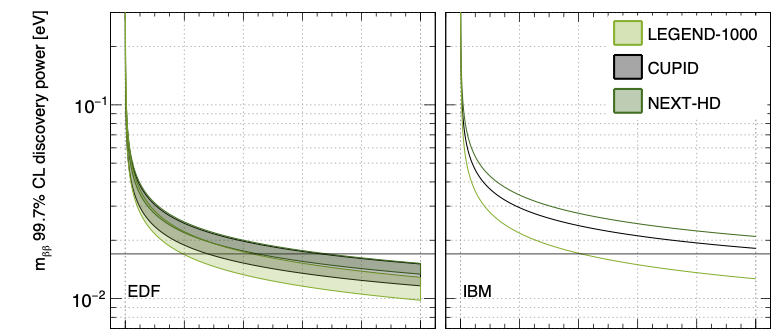
\includegraphics[width=0.55\textwidth]{img/sensiNME.png}
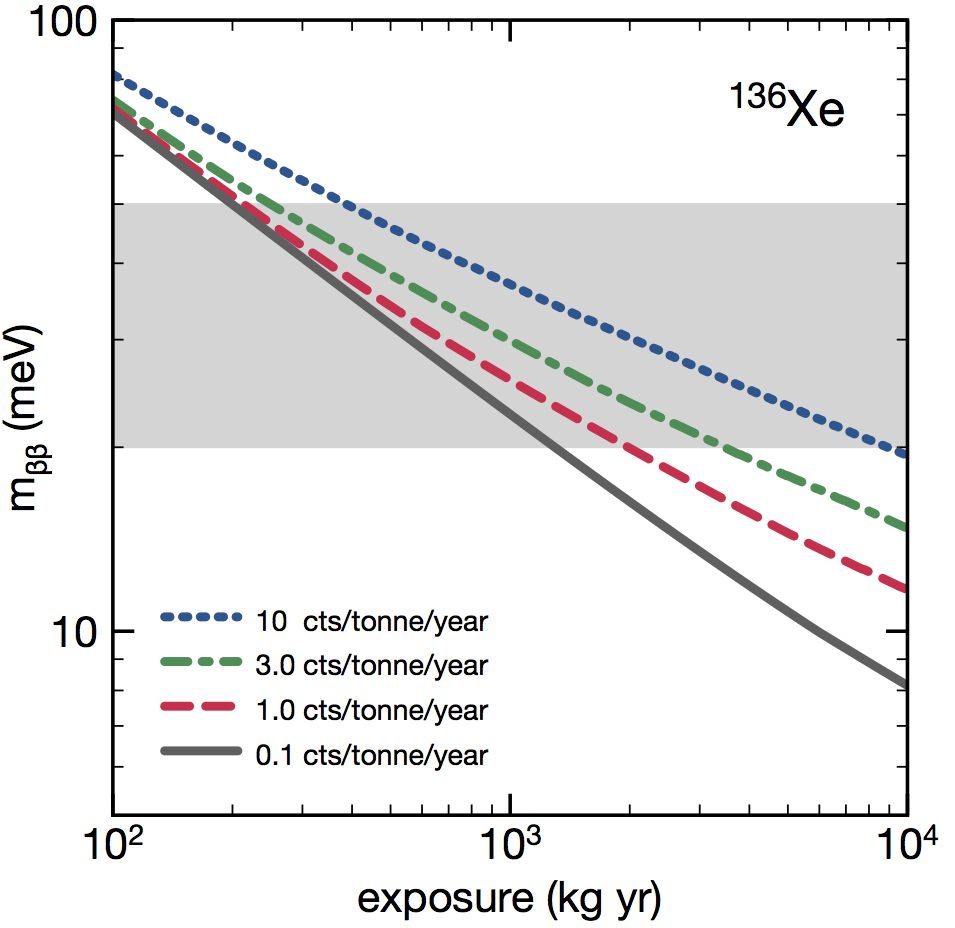
\includegraphics[width=0.35\textwidth]{img/sensi-xenon.png}
\caption{\small Left: the effective neutrino mass \mbb\ as a function of the mass of the lightest neutrino. The current generation of experiments is exploring the so-called ``degenerate neutrino mass region'', up to $\mbb \simeq \SI{50}{\meV}$.  The target of the next generation is to explore the inverse hierarchy, in the range from \SIrange{20}{50}{\meV}. Right: Sensitivity of a fully efficient \XE\ experiment as a function of the exposure, for different background rates.}
\label{fig:Majorana-Landscape}
\end{figure}

The only practical way to determine whether neutrinos are Majorana particles, identical to their own antiparticles, is to observe neutrinoless double beta decay (\bbonu). This is a nuclear transition, $(Z,A) \rightarrow (Z+2,A) + 2\ e^{-}$, in which a nucleus with $Z$ protons decays into a nucleus with $Z+2$ protons and the same mass number $A$, {\em without emitting neutrinos}. The simplest mechanism to mediate such a transition is the virtual exchange of light Majorana neutrinos. Assuming this exchange to be  dominant at low energies, the half-life of \bbonu\ can be written as:

\begin{equation}
(T^{0\nu}_{1/2})^{-1} = G^{0\nu} \ \big|M^{0\nu}\big|^{2} \ \mbb^{2}; \,\,\, \,\,
\mbb = \Big| \sum_{i} U^{2}_{ei} \ m_{i} \Big|
\label{eq:mbb}
\end{equation}
%
where $G^{0\nu}$~ is a phase-space integral for the emission of two electrons, $M^{0\nu}$ is a nuclear matrix element (NME), and \mbb\ is the \emph{effective Majorana mass} of the electron neutrino, defined in terms of the neutrino mass eigenstates ($m_{i}$) and the elements of the neutrino mixing matrix ($U_{ei}$).

When \mbb\ is represented as a function of the lightest neutrino mass, ${\rm m_{light}}$~as in the left panel of Fig.~\ref{fig:Majorana-Landscape}, one obtains the ``Majorana landscape'' defining the space of opportunity for discovery. This landscape is being explored by the current generation of \bbonu\ experiments, achieving exposures in the range of hundred to few hundred kilogram$\cdot$years \cite{Gomez-Cadenas:2019sfa}. Two experiments, one using \GE\ as isotope, and the other using \XE, have achieved the best sensitivity to \Tonu, which is, in both case of the order 
of $10^{26}$ years, finding no signal. These are GERDA~\cite{Agostini:2018tnm}, and KamLAND-Zen~\cite{Gando:2016ji}. As will be discussed later, 
the \Next\ experiment can reach a sensitivity to \Tonu\ similar to that achieved by  KamLAND-Zen, but with a very different systematic error. KamLAND-Zen boasts the largest exposure achieved so far by any \bbonu\ experiment (in excess of one ton$\cdot$year), but also the largest background rate, which needs to be subtracted from the data to search for a putative signal. Instead, \Next\ is expected to be near background-free at the 100 kg scale.

The next step for the field is to extend the sensitivity to \Tonu\ to explore the so-called ``inverted hierarchy'' ordering of neutrino masses, corresponding to the range  \SIrange{20}{50}{\meV} ( left panel of figure \ref{fig:Majorana-Landscape}). To fully cover this region (for most NME),  a sensitivity of, at least,  $10^{27}$ years must be achieved. This, in turn, requires exposures in the range of several \tonne$\cdot$\yr, as well as a dramatic reduction of the background w.r.t. the current standards. 

The detrimental effects of the presence of background are illustrated by the right panel of Figure~\ref{fig:Majorana-Landscape}, which shows the sensitivity to \mbb\ (using a reasonable set of nuclear matrix elements) of a fully efficient \XE\ experiment as a function of exposure, for different background rates.  A fiducial exposure of almost \SI{2}{\tonne\yr} (corresponding to an actual exposure of \SI{5}{\tonne\yr}, when accounting for efficiency of the detector) is required for a full exploration of the IH region {\em in the background free case}, \eg, for \BackgroundFreeLimit\ of background.  The exposure increases to \SI{3}{\tonne\yr} (\SI{8}{\tonne\yr}) for \AlmostBackgroundFreeLimit\ of background and degrades rapidly for larger backgrounds.  Thus, the conclusion is that the next generation of \bbonu\ experiments must feature target masses in the tonne-range, while keeping the total background contained within \AlmostBackgroundFreeRequirement. 
%

The NEXT apparatus can be scaled up to (multi-) tonne target masses, taking advantage of the economy of scale provided by the HPXe technology. Doubling the longitudinal dimensions of \Next\ results in a mass increase of near an order of magnitud ($2^3$), and thus a detector of \SI{200}{cm} diameter and  \SI{300}{cm} length can hold one ton of xenon at a pressure of 15 bar. Douby introducing several new technological advancements \cite{Cadenas:2017vcu}, including: a)  the replacement of PMTs (which are the leading source of background in \Next) with SiPMs, which are intrinsically radiopure, resistant to pressure and able to provide better light collection; b) operation at the detector at \NtkOperatingTemperature, not far from the gas triple point.  Operation in this regime has two marked advantages: i) it reduces the DCR of the SiPMs by a factor \num{300} and b) it permits to operate at a lower pressure (\NtkOperatingPressure) than \Next\ (\NextPressure\ at \NextTemperature).  Reducing the pressure, in turn, simplifies the construction of future larger detectors; c) operation of the detector with a 0.85/0.15 xenon/helium mixture. As shown in Ref.~\cite{Felkai:2017oeq}, the addition of \SI{15}{\percent} of helium reduces the large transverse diffusion of natural xenon gas from \TransverseDiffusionPureXenon\ to \TransverseDiffusionXeHe, resulting in sharper reconstructed images for the electron trajectories and improving the performance of the topological signature by a factor \num{4}~\cite{Renner:2017ey}.
%
%The extrapolation of the technology to the tonne scale could proceed in two stages.  The first stage could upgrade the \NEXT\ detector to turn it into \NHD. This ``high definition detector'' would use a low diffusion gas mixtures and a dense tracking plane to improve the topological signature. The second stage would be \Ntk\, a cool gas xenon TPC operating at \NtkOperatingTemperature\ with a mass of up to \NtkTotalMass\ (\NtkFiducialMass\ fiducial) when the gas is held at a pressure of \NtkMaximumPressure, corresponding to a density of \NtkMaximumDensity.  In addition, if the tantalizing possibility of tagging the \Bapp\ is confirmed \Ntk\ could incorporate a \Bapp\ tagging system. 
%
%%If this proposal is successful, operation of \Next\ is expected to start in 2020. After a physics run of one year, \Next\ will already reach a very competitive sensitivity of \SI{3E+25}{\year} in \Tonu. The \NHD\ detector could reach a sensitivity \SI{3E+26}{\year} in \Tonu\ by 2024 leading the field and perhaps hitting an early discovery. Otherwise, we envision the following jump in the technology (\Ntk) to start in 2025, with the aim of fully exploring the IH, with a great likelihood of discovery.
%
